\documentclass[11pt]{article}
\usepackage[notes]{la}
\lamodule{6}{3}{Orthogonal Projections}
\laxdoc{2.1}
\laxdoc{4.4}
\laxdoc{6.1}
\laxdoc{6.2}

\begin{document}

\section{Orthogonal Projections}

\begin{guide}
In Example~\ref{6.2-ex:notin} the weight formula was applied to a vector $\bv{y}$ that was \emph{not} in the span of an orthogonal set. It did not fail: it produced a vector of the span, and the leftover $\bv{y}-(\text{that vector})$ turned out to be perpendicular to every vector of the set. This section turns that observation into a theorem. For any subspace $W$ that has an orthogonal basis, every $\bv{y}$ splits in exactly one way into a part in $W$ and a part in $W^{\perp}$. The part in $W$ is the \emph{orthogonal projection} of $\bv{y}$ onto $W$, and it is the point of $W$ closest to $\bv{y}$. That second fact is the one that makes projections useful: whenever a vector must be replaced by one from a smaller set, the projection is the best replacement.
\end{guide}

\textbf{By the end of this section you should be able to:}
\begin{itemize}
  \item split a vector $\bv{y}$ as $\hat{\bv{y}}+\bv{z}$ with $\hat{\bv{y}}$ in a subspace $W$ and $\bv{z}$ in $W^{\perp}$, and explain why the split is unique;
  \item compute $\proj_W\bv{y}$ from an orthogonal basis of $W$ with the dot-product formula;
  \item find the closest point of $W$ to $\bv{y}$ and the distance from $\bv{y}$ to $W$, and justify that no other point is closer;
  \item write $\proj_W\bv{y}=UU\T\bv{y}$ when the columns of $U$ are an orthonormal basis of $W$, and recognise the properties of the matrix $UU\T$;
  \item read the split in coordinates: the weights of $\bv{y}$ in an orthogonal basis of $\R^n$ that begins with a basis of $W$.
\end{itemize}

% ---------------------------------------------------------------------
\subsection*{Splitting a vector into a part in $W$ and a part in $W^{\perp}$}

Recall that $W^{\perp}$ is the set of all vectors orthogonal to every vector of $W$ (Definition~\ref{6.1-def:perp}), and that to test $\bv{x}$ for membership in $W^{\perp}$ it is enough to dot it with a spanning set of $W$ (Theorem~\ref{6.1-thm:perpfacts}(a)).

\begin{exmp}{Picking up where Section 6.2 stopped}{revisit}
Let $\bv{a}_1=(1,1,1)$, $\bv{a}_2=(1,-2,1)$, $W=\Span\{\bv{a}_1,\bv{a}_2\}$ and $\bv{y}=(2,1,3)$, as in Example~\ref{6.2-ex:notin}. The formula gave the combination $\tfrac{6}{3}\bv{a}_1+\tfrac{3}{6}\bv{a}_2=(\tfrac52,1,\tfrac52)$, which is in $W$, and the leftover $\bv{y}-(\tfrac52,1,\tfrac52)=(-\tfrac12,0,\tfrac12)$. Is the leftover in $W^{\perp}$? Dot it with the two spanning vectors: $-\tfrac12+0+\tfrac12=0$ and $-\tfrac12-0+\tfrac12=0$. By Theorem~\ref{6.1-thm:perpfacts}(a) it is in $W^{\perp}$. So
\[
(2,1,3)=\underbrace{(\tfrac52,1,\tfrac52)}_{\text{in }W}+\underbrace{(-\tfrac12,0,\tfrac12)}_{\text{in }W^{\perp}} .
\]
\end{exmp}

In Section 6.2 we knew the leftover was perpendicular because it was a multiple of a third basis vector $\bv{a}_3$. The theorem below needs no third vector at all.

\begin{exmp}{Grouping the terms of an expansion}{group}
Take the full orthogonal basis $\bv{a}_1=(1,1,1)$, $\bv{a}_2=(1,-2,1)$, $\bv{a}_3=(1,0,-1)$ of $\R^3$ and $\bv{y}=(4,4,-2)=2\bv{a}_1-\bv{a}_2+3\bv{a}_3$ (the weights were found in Example~\ref{6.2-ex:weights1}). Let $W=\Span\{\bv{a}_1,\bv{a}_2\}$. Group the terms:
\[
\bv{y}=\underbrace{(2\bv{a}_1-\bv{a}_2)}_{=(1,4,1)\text{ in }W}+\underbrace{3\bv{a}_3}_{=(3,0,-3)} .
\]
The second part is orthogonal to $W$: $(3,0,-3)\cdot\bv{a}_1=3+0-3=0$ and $(3,0,-3)\cdot\bv{a}_2=3+0-3=0$. So grouping an orthogonal expansion always gives a split of $\bv{y}$ into a vector of $W$ and a vector of $W^{\perp}$.
\end{exmp}

Grouping works only because we had a basis for all of $\R^3$. The next theorem gets the same split from a basis of $W$ alone.

\begin{thm}{The Orthogonal Decomposition Theorem}{decomp}
Let $W$ be a subspace of $\R^n$ and let $\bv{y}$ be in $\R^n$.
\begin{enumerate}[label=(\alph*),itemsep=1pt]
  \item \emph{Uniqueness.} There is at most one way to write $\bv{y}=\hat{\bv{y}}+\bv{z}$ with $\hat{\bv{y}}$ in $W$ and $\bv{z}$ in $W^{\perp}$.
  \item \emph{Existence.} If $W$ has an orthogonal basis $\bv{u}_1,\dots,\bv{u}_p$ (all nonzero), then such a split exists, namely
\[
\hat{\bv{y}}=\frac{\bv{y}\cdot\bv{u}_1}{\bv{u}_1\cdot\bv{u}_1}\bv{u}_1+\cdots+\frac{\bv{y}\cdot\bv{u}_p}{\bv{u}_p\cdot\bv{u}_p}\bv{u}_p,\qquad\bv{z}=\bv{y}-\hat{\bv{y}} .
\]
\end{enumerate}
\end{thm}

\begin{proof}
(b)~Define $\hat{\bv{y}}$ by the formula. It is a combination of the basis vectors, so it lies in $W$, and $\hat{\bv{y}}+\bv{z}=\bv{y}$ by the definition of $\bv{z}$. Next dot $\bv{z}$ with $\bv{u}_1$. Because $\bv{u}_1\cdot\bv{u}_j=0$ for $j\neq1$, only the first term of $\hat{\bv{y}}$ survives:
\[
\bv{z}\cdot\bv{u}_1=\bv{y}\cdot\bv{u}_1-\frac{\bv{y}\cdot\bv{u}_1}{\bv{u}_1\cdot\bv{u}_1}(\bv{u}_1\cdot\bv{u}_1)=0 .
\]
The same computation gives $\bv{z}\cdot\bv{u}_j=0$ for every $j$, so $\bv{z}$ is in $W^{\perp}$ by Theorem~\ref{6.1-thm:perpfacts}(a).

(a)~Suppose $\bv{y}=\hat{\bv{y}}_1+\bv{z}_1=\hat{\bv{y}}_2+\bv{z}_2$ are two splits. Then $\bv{v}=\hat{\bv{y}}_1-\hat{\bv{y}}_2=\bv{z}_2-\bv{z}_1$. The left side is in $W$ (a difference of vectors of $W$) and the right side is in $W^{\perp}$ (a subspace, Theorem~\ref{6.1-thm:perpfacts}(b)). So $\bv{v}$ is orthogonal to itself: $\bv{v}\cdot\bv{v}=0$, hence $\bv{v}=\bv{0}$ by Theorem~\ref{6.1-thm:dotprops}. Thus $\hat{\bv{y}}_1=\hat{\bv{y}}_2$ and $\bv{z}_1=\bv{z}_2$.
\end{proof}

Part (a) holds for \emph{every} subspace. Part (b) needs an orthogonal basis, and so far we only have one when someone hands it to us (as in Section 6.2) or when we can find it by hand (Example~\ref{ex:build} below). A later section shows that every subspace of $\R^n$ has an orthogonal basis; until then, ``a subspace $W$'' in this section means a nonzero subspace that comes with an orthogonal basis. The next definition gives the part in $W$ a name.

\begin{defn}{Orthogonal projection onto a subspace}{projW}
Let $W$ be a subspace for which $\bv{y}=\hat{\bv{y}}+\bv{z}$ with $\hat{\bv{y}}$ in $W$ and $\bv{z}$ in $W^{\perp}$ exists. The vector $\hat{\bv{y}}$ is the \emph{orthogonal projection of $\bv{y}$ onto $W$}, written $\proj_W\bv{y}$. The vector $\bv{z}=\bv{y}-\proj_W\bv{y}$ is the \emph{component of $\bv{y}$ orthogonal to $W$}.
\end{defn}

By Theorem~\ref{thm:decomp}(a) the vector $\proj_W\bv{y}$ depends only on $W$ and $\bv{y}$, not on which orthogonal basis was used to compute it (Pause and think~\ref{think:twobases}). For a line $W=L=\Span\{\bv{u}\}$ the formula has one term and is the one of Definition~\ref{6.2-def:proj}.

\begin{center}
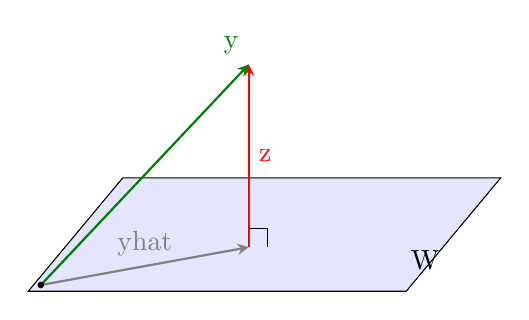
\begin{tikzpicture}[>=stealth,scale=0.8]
  \draw[fill=blue!10] (0,0)--(6,0)--(7.5,1.8)--(1.5,1.8)--cycle;
  \node at (6.3,0.5) {W};
  \draw[->,thick,red] (3.5,0.7)--(3.5,3.6) node[midway,right] {z};
  \draw[->,thick,gray] (0.2,0.1)--(3.5,0.7) node[midway,above] {yhat};
  \draw[->,thick,green!50!black] (0.2,0.1)--(3.5,3.6) node[above left] {y};
  \draw (3.5,1.0)--(3.8,1.0)--(3.8,0.7);
  \fill (0.2,0.1) circle (1.5pt);
\end{tikzpicture}
\end{center}

\noindent\textbf{Figure 1.} The vector $\bv{y}$ is the hypotenuse of a right triangle: $\hat{\bv{y}}=\proj_W\bv{y}$ lies in the plane $W$ and $\bv{z}$ is perpendicular to $W$.

\begin{proc}{Projection onto $W$ from an orthogonal basis}{projproc}
Given an orthogonal basis $\bv{u}_1,\dots,\bv{u}_p$ for $W$ and a vector $\bv{y}$:
\begin{enumerate}[nosep]
  \item test every pair: $\bv{u}_i\cdot\bv{u}_j=0$ for $i\neq j$ (the formula is wrong if one pair fails);
  \item compute the denominators $\bv{u}_j\cdot\bv{u}_j$ and the numerators $\bv{y}\cdot\bv{u}_j$;
  \item form $\hat{\bv{y}}=\sum_j\frac{\bv{y}\cdot\bv{u}_j}{\bv{u}_j\cdot\bv{u}_j}\bv{u}_j$ and $\bv{z}=\bv{y}-\hat{\bv{y}}$;
  \item check that $\bv{z}\cdot\bv{u}_j=0$ for every $j$.
\end{enumerate}
\end{proc}

\begin{exmp}{Projection onto a plane in $\R^3$}{plane3}
Let $\bv{p}_1=(1,2,2)$, $\bv{p}_2=(2,1,-2)$ and $W=\Span\{\bv{p}_1,\bv{p}_2\}$, and let $\bv{y}=(3,3,3)$. The pair is orthogonal: $\bv{p}_1\cdot\bv{p}_2=2+2-4=0$, and $\bv{p}_1\cdot\bv{p}_1=9=\bv{p}_2\cdot\bv{p}_2$. The numerators are $\bv{y}\cdot\bv{p}_1=3+6+6=15$ and $\bv{y}\cdot\bv{p}_2=6+3-6=3$. So
\[
\hat{\bv{y}}=\tfrac{15}{9}(1,2,2)+\tfrac39(2,1,-2)=(\tfrac53+\tfrac23,\ \tfrac{10}3+\tfrac13,\ \tfrac{10}3-\tfrac23)=(\tfrac73,\tfrac{11}3,\tfrac83),\qquad\bv{z}=(\tfrac23,-\tfrac23,\tfrac13).
\]
Check: $\bv{z}\cdot\bv{p}_1=\tfrac23-\tfrac43+\tfrac23=0$ and $\bv{z}\cdot\bv{p}_2=\tfrac43-\tfrac23-\tfrac23=0$. \ $\checkmark$
\end{exmp}

\begin{exmp}{A subspace of $\R^4$}{r4}
Let $\bv{t}_1=(1,-2,-1,0)$ and $\bv{t}_2=(1,0,1,-1)$, so $\bv{t}_1\cdot\bv{t}_2=1+0-1+0=0$, with $\bv{t}_1\cdot\bv{t}_1=6$ and $\bv{t}_2\cdot\bv{t}_2=3$. For $\bv{y}=(5,0,2,1)$ we get $\bv{y}\cdot\bv{t}_1=5-0-2+0=3$ and $\bv{y}\cdot\bv{t}_2=5+0+2-1=6$. Hence
\[
\hat{\bv{y}}=\tfrac36(1,-2,-1,0)+\tfrac63(1,0,1,-1)=(\tfrac52,-1,\tfrac32,-2),\qquad\bv{z}=\bv{y}-\hat{\bv{y}}=(\tfrac52,1,\tfrac12,3).
\]
Check: $\bv{z}\cdot\bv{t}_1=\tfrac52-2-\tfrac12+0=0$ and $\bv{z}\cdot\bv{t}_2=\tfrac52+0+\tfrac12-3=0$. \ $\checkmark$ Nothing in the method depends on the number of entries: only dot products are used.
\end{exmp}

\begin{exmp}{A vector already in $W$}{inW}
With $W$ as in Example~\ref{ex:plane3}, let $\bv{y}=(5,4,-2)$. Then $\bv{y}\cdot\bv{p}_1=5+8-4=9$ and $\bv{y}\cdot\bv{p}_2=10+4+4=18$, so $\hat{\bv{y}}=1\cdot\bv{p}_1+2\cdot\bv{p}_2=(5,4,-2)=\bv{y}$ and $\bv{z}=\bv{0}$. When $\bv{y}$ is in $W$ the projection returns $\bv{y}$ itself, and the weights are the ones of Theorem~\ref{6.2-thm:weights}.
\end{exmp}

\begin{exmp}{A vector perpendicular to $W$}{perpW}
With the same $W$ let $\bv{y}=(4,-4,2)$. Then $\bv{y}\cdot\bv{p}_1=4-8+4=0$ and $\bv{y}\cdot\bv{p}_2=8-4-4=0$, so $\hat{\bv{y}}=\bv{0}$ and $\bv{z}=\bv{y}$. The vector is in $W^{\perp}$ and its projection onto $W$ is zero.
\end{exmp}

\begin{thm}{Properties of the projection}{projprops}
Let $W$ be a subspace of $\R^n$ for which projections exist.
\begin{enumerate}[label=(\alph*),itemsep=1pt]
  \item $\proj_W\bv{y}=\bv{y}$ if and only if $\bv{y}$ is in $W$; and $\proj_W\bv{y}=\bv{0}$ if and only if $\bv{y}$ is in $W^{\perp}$.
  \item $\proj_W(\bv{y}_1+\bv{y}_2)=\proj_W\bv{y}_1+\proj_W\bv{y}_2$ and $\proj_W(c\bv{y})=c\,\proj_W\bv{y}$.
  \item $\proj_W(\proj_W\bv{y})=\proj_W\bv{y}$: projecting twice is the same as projecting once.
\end{enumerate}
\end{thm}

\begin{proof}
(a)~If $\bv{y}$ is in $W$, then $\bv{y}=\bv{y}+\bv{0}$ is a split with the first part in $W$ and $\bv{0}$ in $W^{\perp}$, so by uniqueness (Theorem~\ref{thm:decomp}(a)) $\proj_W\bv{y}=\bv{y}$. Conversely, $\proj_W\bv{y}$ is in $W$ by definition. If $\bv{y}$ is in $W^{\perp}$, then $\bv{y}=\bv{0}+\bv{y}$ is a split, so $\proj_W\bv{y}=\bv{0}$. Conversely, if $\proj_W\bv{y}=\bv{0}$ then $\bv{y}=\bv{0}+\bv{z}$ with $\bv{z}$ in $W^{\perp}$.

(b)~Let $\bv{y}_1=\hat{\bv{y}}_1+\bv{z}_1$ and $\bv{y}_2=\hat{\bv{y}}_2+\bv{z}_2$ be the splits. Then $\bv{y}_1+\bv{y}_2=(\hat{\bv{y}}_1+\hat{\bv{y}}_2)+(\bv{z}_1+\bv{z}_2)$ with the first part in $W$ and the second in $W^{\perp}$, because both are subspaces. By uniqueness this is the split of $\bv{y}_1+\bv{y}_2$. The same argument works for $c\bv{y}=c\hat{\bv{y}}+c\bv{z}$.

(c)~$\proj_W\bv{y}$ is in $W$, so part (a) says that projecting it returns it.
\end{proof}

\begin{exmp}{Projecting a sum}{linear}
Use $W$ from Example~\ref{ex:plane3}. We found $\proj_W(3,3,3)=(\tfrac73,\tfrac{11}3,\tfrac83)$. For $\bv{y}_2=(6,0,3)$: $\bv{y}_2\cdot\bv{p}_1=6+0+6=12$ and $\bv{y}_2\cdot\bv{p}_2=12+0-6=6$, so $\proj_W\bv{y}_2=\tfrac{12}9\bv{p}_1+\tfrac69\bv{p}_2=(\tfrac83,\tfrac{10}3,\tfrac43)$. The sum of the two projections is $(5,7,4)$. Directly, $\bv{y}_1+\bv{y}_2=(9,3,6)$ has numerators $9+6+12=27$ and $18+3-12=9$, so its projection is $3\bv{p}_1+1\bv{p}_2=(5,7,4)$. \ $\checkmark$
\end{exmp}

\begin{think}{Where did the third vector go?}{leftover}
In Example~\ref{ex:revisit} the leftover $(-\tfrac12,0,\tfrac12)$ was a multiple of $\bv{a}_3=(1,0,-1)$, which is orthogonal to $\bv{a}_1$ and $\bv{a}_2$. Theorem~\ref{thm:decomp} produces a perpendicular leftover from $\bv{a}_1,\bv{a}_2$ alone. Why is there no contradiction? What would the leftover be if $\bv{y}$ were a multiple of $\bv{a}_3$?
\end{think}

\begin{think}{Two orthogonal bases for one plane}{twobases}
Check that $\bv{q}_1=\bv{p}_1+\bv{p}_2$ and $\bv{q}_2=\bv{p}_1-\bv{p}_2$ are orthogonal and span the same plane $W$ as $\bv{p}_1,\bv{p}_2$. Compute $\proj_W(3,3,3)$ with $\bv{q}_1,\bv{q}_2$ and compare with Example~\ref{ex:plane3}. Which part of Theorem~\ref{thm:decomp} explains the result?
\end{think}

\begin{kc}{Splitting a vector}{kcsplit}
Let $W=\Span\{(1,1,0),(1,-1,0)\}$ and $\bv{y}=(3,5,7)$. Find $\proj_W\bv{y}$ and $\bv{z}$, and check that $\bv{z}$ is orthogonal to both basis vectors.
\end{kc}

\begin{kc}{Is the vector in $W$?}{kcinw}
Let $W=\Span\{(1,1,1),(1,-2,1)\}$. Compute $\proj_W\bv{y}$ for $\bv{y}=(3,0,3)$ and decide from the answer whether $\bv{y}$ is in $W$. Which part of Theorem~\ref{thm:projprops} are you using?
\end{kc}

% ---------------------------------------------------------------------
\subsection*{Building an orthogonal basis by hand, and when the formula fails}

The formula needs an orthogonal basis. If a plane is given by an equation, we can build one directly: pick one vector in the plane, then find a second vector that lies in the plane \emph{and} is perpendicular to the first. Both requirements are dot-product equations, so this is a homogeneous system.

\begin{exmp}{An orthogonal basis for a plane given by an equation}{build}
The plane $H=\{\bv{x}:\ x_1-2x_2+x_3=0\}$ of Example~\ref{4.4-ex:plane} contains $\bv{u}_1=(2,1,0)$, since $2-2+0=0$. A vector $\bv{u}_2$ of $H$ that is orthogonal to $\bv{u}_1$ satisfies $x_1-2x_2+x_3=0$ and $2x_1+x_2=0$:
\[
\begin{amat}{ccc}1&-2&1\\2&1&0\end{amat}\rops{R_2-2R_1}\begin{amat}{ccc}1&-2&1\\0&5&-2\end{amat}\rops{\frac15R_2}\begin{amat}{ccc}1&-2&1\\0&1&-\frac25\end{amat}\rops{R_1+2R_2}\begin{amat}{ccc}1&0&\frac15\\0&1&-\frac25\end{amat}.
\]
So $x_1=-\tfrac15x_3$ and $x_2=\tfrac25x_3$; with $x_3=-5$ we get $\bv{u}_2=(1,-2,-5)$. Check: $1+4-5=0$, so $\bv{u}_2$ is in $H$, and $\bv{u}_1\cdot\bv{u}_2=2-2+0=0$. \ $\checkmark$ Now project $\bv{y}=(1,0,0)$ onto $H$. We have $\bv{u}_1\cdot\bv{u}_1=5$, $\bv{u}_2\cdot\bv{u}_2=30$, $\bv{y}\cdot\bv{u}_1=2$ and $\bv{y}\cdot\bv{u}_2=1$, so
\[
\hat{\bv{y}}=\tfrac25(2,1,0)+\tfrac1{30}(1,-2,-5)=(\tfrac56,\tfrac13,-\tfrac16),\qquad\bv{z}=(\tfrac16,-\tfrac13,\tfrac16)=\tfrac16(1,-2,1).
\]
The leftover is a multiple of $(1,-2,1)$, the vector of coefficients of the equation of $H$; this is what we should expect, since the coefficients of the equation are the entries of a vector orthogonal to $H$ (Theorem~\ref{6.1-thm:rowcolperp}).
\end{exmp}

\begin{warn}[Orthogonal basis needed]
If the spanning vectors are not orthogonal, the formula of Theorem~\ref{thm:decomp}(b) gives a vector of $W$ but \emph{not} the projection.
\end{warn}

\begin{exmp}{The formula with a basis that is not orthogonal}{wrong}
Let $\bv{b}_1=(1,0,1)$, $\bv{b}_2=(1,1,0)$ and $\bv{y}=(1,2,3)$. Here $\bv{b}_1\cdot\bv{b}_2=1\neq0$. The formula (misused) gives $\tfrac42\bv{b}_1+\tfrac32\bv{b}_2=(\tfrac72,\tfrac32,2)$ and $\bv{y}-(\tfrac72,\tfrac32,2)=(-\tfrac52,\tfrac12,1)$, whose dot product with $\bv{b}_1$ is $-\tfrac52+1=-\tfrac32\neq0$: not perpendicular to $W$. The repair is to replace $\bv{b}_2$ by a vector of $W$ orthogonal to $\bv{b}_1$. The vector $2\bv{b}_2-\bv{b}_1=(1,2,-1)$ is in $W$ and $(1,2,-1)\cdot\bv{b}_1=1-1=0$. With this orthogonal basis, $\bv{y}\cdot\bv{b}_1=4$ and $\bv{y}\cdot(1,2,-1)=1+4-3=2$, so
\[
\hat{\bv{y}}=\tfrac42(1,0,1)+\tfrac26(1,2,-1)=(\tfrac73,\tfrac23,\tfrac53),\qquad\bv{z}=(-\tfrac43,\tfrac43,\tfrac43).
\]
Check: $\bv{z}\cdot\bv{b}_1=-\tfrac43+\tfrac43=0$ and $\bv{z}\cdot(1,2,-1)=-\tfrac43+\tfrac83-\tfrac43=0$. \ $\checkmark$
\end{exmp}

\begin{think}{The whole space}{allofspace}
(a)~What is $\proj_W\bv{y}$ when $W=\R^n$ and $\bv{u}_1,\dots,\bv{u}_n$ is an orthogonal basis of $\R^n$? (b)~What are $\proj_W\bv{y}$ and $\bv{z}$ when $W$ is the line $\Span\{\bv{u}\}$ and $\bv{y}$ is a multiple of $\bv{u}$?
\end{think}

% ---------------------------------------------------------------------
\subsection*{The split in coordinates}

Let $\mathcal{B}=\{\bv{p}_1,\bv{p}_2,\bv{p}_3\}$ with $\bv{p}_3=(2,-2,1)$. All three pairs are orthogonal, so $\mathcal{B}$ is an orthogonal basis of $\R^3$ and the coordinates of any $\bv{y}$ relative to $\mathcal{B}$ (Definition~\ref{4.4-def:coords}) are the weights $c_j=\bv{y}\cdot\bv{p}_j/9$ of Theorem~\ref{6.2-thm:weights}.

\begin{exmp}{Projection reads off two coordinates}{coordsP}
For $\bv{y}=(3,3,3)$ the numerators are $15$, $3$ and $\bv{y}\cdot\bv{p}_3=6-6+3=3$, so $[\bv{y}]_{\mathcal{B}}=(\tfrac53,\tfrac13,\tfrac13)$. With $W=\Span\{\bv{p}_1,\bv{p}_2\}$, Example~\ref{ex:plane3} gave $\hat{\bv{y}}=\tfrac53\bv{p}_1+\tfrac13\bv{p}_2$ and $\bv{z}=\tfrac13\bv{p}_3=(\tfrac23,-\tfrac23,\tfrac13)$. In coordinates:
\[
[\bv{y}]_{\mathcal{B}}=(\tfrac53,\tfrac13,\tfrac13),\qquad[\hat{\bv{y}}]_{\mathcal{B}}=(\tfrac53,\tfrac13,0),\qquad[\bv{z}]_{\mathcal{B}}=(0,0,\tfrac13).
\]
Projecting onto $W$ keeps the first two coordinates and sets the third to $0$.
\end{exmp}

\begin{think}{Which coordinate measures the distance}{coordsmeaning}
In Example~\ref{ex:coordsP}, which coordinate of $\bv{y}$ measures how far $\bv{y}$ is from $W$, and why does it equal $\lVert\bv{z}\rVert$ divided by $\lVert\bv{p}_3\rVert$?
\end{think}

% ---------------------------------------------------------------------
\subsection*{The closest point of $W$}

\begin{thm}{The Best Approximation Theorem}{best}
Let $W$ be a subspace of $\R^n$ for which projections exist, let $\bv{y}$ be in $\R^n$ and let $\hat{\bv{y}}=\proj_W\bv{y}$. Then for every $\bv{v}$ in $W$ with $\bv{v}\neq\hat{\bv{y}}$,
\[
\lVert\bv{y}-\hat{\bv{y}}\rVert<\lVert\bv{y}-\bv{v}\rVert .
\]
That is, $\hat{\bv{y}}$ is the unique point of $W$ closest to $\bv{y}$.
\end{thm}

\begin{proof}
Write $\bv{y}-\bv{v}=(\bv{y}-\hat{\bv{y}})+(\hat{\bv{y}}-\bv{v})$. The vector $\hat{\bv{y}}-\bv{v}$ is in $W$, because $\hat{\bv{y}}$ and $\bv{v}$ are. The vector $\bv{y}-\hat{\bv{y}}=\bv{z}$ is orthogonal to every vector of $W$, in particular to $\hat{\bv{y}}-\bv{v}$. By the Pythagorean theorem (Theorem~\ref{6.1-thm:pyth}),
\[
\lVert\bv{y}-\bv{v}\rVert^2=\lVert\bv{y}-\hat{\bv{y}}\rVert^2+\lVert\hat{\bv{y}}-\bv{v}\rVert^2 .
\]
Since $\bv{v}\neq\hat{\bv{y}}$, the last term is positive. Hence $\lVert\bv{y}-\bv{v}\rVert^2>\lVert\bv{y}-\hat{\bv{y}}\rVert^2$, and taking square roots gives the claim.
\end{proof}

\begin{center}
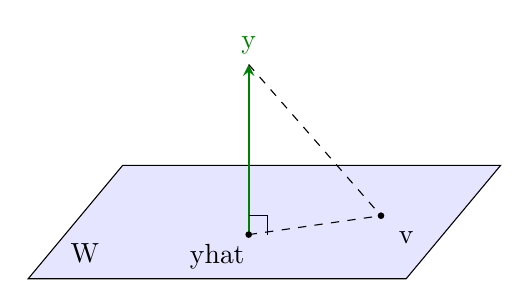
\begin{tikzpicture}[>=stealth,scale=0.8]
  \draw[fill=blue!10] (0,0)--(6,0)--(7.5,1.8)--(1.5,1.8)--cycle;
  \node at (0.9,0.4) {W};
  \draw[->,thick,green!50!black] (3.5,0.7)--(3.5,3.4) node[above] {y};
  \fill (3.5,0.7) circle (1.5pt);
  \node at (3.0,0.35) {yhat};
  \fill (5.6,1.0) circle (1.5pt);
  \node at (6.0,0.65) {v};
  \draw[dashed] (3.5,3.4)--(5.6,1.0);
  \draw[dashed] (3.5,0.7)--(5.6,1.0);
  \draw (3.5,1.0)--(3.8,1.0)--(3.8,0.7);
\end{tikzpicture}
\end{center}

\noindent\textbf{Figure 2.} The segment from $\bv{y}$ to $\hat{\bv{y}}$ is perpendicular to $W$, so it is the shortest segment from $\bv{y}$ to the plane. For any other point $\bv{v}$ of $W$ the segment from $\bv{y}$ to $\bv{v}$ is the hypotenuse of a right triangle.

\begin{defn}{Distance from a vector to a subspace}{dist}
The \emph{distance from $\bv{y}$ to $W$} is the length $\lVert\bv{y}-\proj_W\bv{y}\rVert$ of the component of $\bv{y}$ orthogonal to $W$. By Theorem~\ref{thm:best} no point of $W$ is nearer to $\bv{y}$.
\end{defn}

\begin{exmp}{The closest point and a competitor}{best}
Use $W$ from Example~\ref{ex:plane3} and $\bv{y}=(6,0,3)$. We found $\proj_W\bv{y}=(\tfrac83,\tfrac{10}3,\tfrac43)$, so $\bv{z}=(\tfrac{10}3,-\tfrac{10}3,\tfrac53)$ and $\lVert\bv{z}\rVert^2=\tfrac{100+100+25}9=25$. The distance from $\bv{y}$ to $W$ is $5$. Now try the point $\bv{v}=\bv{p}_1+\bv{p}_2=(3,3,0)$ of $W$. Then $\bv{y}-\bv{v}=(3,-3,3)$ with $\lVert\bv{y}-\bv{v}\rVert^2=27$, which exceeds $25$. The Pythagorean relation of the proof holds: $\hat{\bv{y}}-\bv{v}=(-\tfrac13,\tfrac13,\tfrac43)$ has squared length $\tfrac{1+1+16}9=2$, and $25+2=27$. \ $\checkmark$
\end{exmp}

\begin{exmp}{Two ways to the same distance}{twoways}
With $W$, $\bv{y}=(6,0,3)$ as above, the third vector $\bv{p}_3=(2,-2,1)$ is orthogonal to $\bv{p}_1$ and $\bv{p}_2$, and grouping the expansion of $\bv{y}$ in $\{\bv{p}_1,\bv{p}_2,\bv{p}_3\}$ (Example~\ref{ex:coordsP}) shows $\bv{z}=c_3\bv{p}_3$ with $c_3=\bv{y}\cdot\bv{p}_3/9=15/9=\tfrac53$. So $\lVert\bv{z}\rVert=\tfrac53\lVert\bv{p}_3\rVert=\tfrac53\cdot3=5$, the same distance as above: $|\bv{y}\cdot\bv{p}_3|/\lVert\bv{p}_3\rVert=15/3=5$. When $W^{\perp}$ is a line, the distance can be found from one dot product.
\end{exmp}

\begin{think}{A point of $W$ is a point of $W$}{closure}
In the proof of Theorem~\ref{thm:best}, why is $\hat{\bv{y}}-\bv{v}$ in $W$? Which property of a subspace is used?
\end{think}

\begin{kc}{A distance}{kcdist}
For $W=\Span\{\bv{p}_1,\bv{p}_2\}$ as in Example~\ref{ex:plane3} and $\bv{y}=(9,3,3)$, find $\proj_W\bv{y}$ and the distance from $\bv{y}$ to $W$.
\end{kc}

\begin{think}{Two vectors, one distance}{samedist}
In Knowledge Check~\ref{kc:kcdist} the distance equals the one in Example~\ref{ex:best}, although $(9,3,3)\neq(6,0,3)$. Compare the two vectors. Why must they have the same component orthogonal to $W$?
\end{think}

% ---------------------------------------------------------------------
\subsection*{Orthonormal bases and the matrix $UU\T$}

\begin{thm}{Projection with an orthonormal basis}{orthonormal}
Let $\bv{u}_1,\dots,\bv{u}_p$ be an orthonormal basis for $W$ and $U=\begin{bmatrix}\bv{u}_1&\cdots&\bv{u}_p\end{bmatrix}$. Then for every $\bv{y}$ in $\R^n$
\[
\proj_W\bv{y}=(\bv{y}\cdot\bv{u}_1)\bv{u}_1+\cdots+(\bv{y}\cdot\bv{u}_p)\bv{u}_p=UU\T\bv{y} .
\]
In particular $\proj_W\bv{y}=U\bv{x}$ for $\bv{x}=U\T\bv{y}$ in $\R^p$.
\end{thm}

\begin{proof}
Each $\bv{u}_j\cdot\bv{u}_j=1$, so the formula of Theorem~\ref{thm:decomp}(b) reduces to the first equality. The entries of $U\T\bv{y}$ are the dot products $\bv{u}_j\cdot\bv{y}$ (row $j$ of $U\T$ is $\bv{u}_j\T$). The product $U(U\T\bv{y})$ is the combination of the columns of $U$ with those entries as weights (Section 1.4), which is $\sum_j(\bv{y}\cdot\bv{u}_j)\bv{u}_j$.
\end{proof}

Recall that $U\T U=I_p$ when the columns of $U$ are orthonormal (Theorem~\ref{6.2-thm:utu}). The other product, $UU\T$, is $n\times n$ and is \emph{not} the identity unless $p=n$.

\begin{exmp}{The matrix of a projection}{projmat}
The vectors $\tfrac13\bv{p}_1$ and $\tfrac13\bv{p}_2$ are an orthonormal basis for $W$ of Example~\ref{ex:plane3}; let $U=\tfrac13\begin{bmatrix}1&2\\2&1\\2&-2\end{bmatrix}$. Then
\[
UU\T=\tfrac19\begin{bmatrix}1&2\\2&1\\2&-2\end{bmatrix}\begin{bmatrix}1&2&2\\2&1&-2\end{bmatrix}=\tfrac19\begin{bmatrix}5&4&-2\\4&5&2\\-2&2&8\end{bmatrix}.
\]
Apply it to $\bv{y}=(3,3,3)$: $UU\T\bv{y}=\tfrac19(15+12-6,\ 12+15+6,\ -6+6+24)=\tfrac19(21,33,24)=(\tfrac73,\tfrac{11}3,\tfrac83)$, the vector found in Example~\ref{ex:plane3}. The projection is a matrix multiplication.
\end{exmp}

\begin{exmp}{Properties of $UU\T$}{pprops}
Let $P=\tfrac19\begin{bmatrix}5&4&-2\\4&5&2\\-2&2&8\end{bmatrix}$ be the matrix of Example~\ref{ex:projmat}. It is symmetric. Its square is $P^2=\tfrac1{81}\begin{bmatrix}45&36&-18\\36&45&18\\-18&18&72\end{bmatrix}=P$, as predicted by Theorem~\ref{thm:projprops}(c). It fixes the vectors of $W$ and kills the vectors of $W^{\perp}$: $P\bv{p}_3=\tfrac19(10-8-2,\ 8-10+2,\ -4-4+8)=(0,0,0)$.
\end{exmp}

\begin{exmp}{When $W$ is everything}{square}
Let $Q=\tfrac13\begin{bmatrix}1&2&2\\2&1&-2\\2&-2&1\end{bmatrix}$. Its columns are an orthonormal basis for $\R^3$, so $QQ\T=I$ (Theorem~\ref{6.2-thm:orthinv}) and $\proj_{\R^3}\bv{y}=\bv{y}$ for every $\bv{y}$. The matrix $UU\T$ is the identity exactly when there are as many columns as rows.
\end{exmp}

\begin{kc}{An orthonormal basis}{kcorthonormal}
The columns of $U=\tfrac12\begin{bmatrix}1&1\\1&1\\1&-1\\1&-1\end{bmatrix}$ are orthonormal. Use Theorem~\ref{thm:orthonormal} to find $\proj_W\bv{y}$ for $\bv{y}=(4,2,6,0)$, where $W=\Col U$.
\end{kc}

\begin{kc}{A projection matrix}{kcmat}
Let $U=\begin{bmatrix}1&0\\0&1\\0&0\end{bmatrix}$. Compute $UU\T$ and describe in words what $UU\T\bv{y}$ does to a vector $\bv{y}=(y_1,y_2,y_3)$.
\end{kc}

\begin{think}{Sizes}{shapes}
For a $3\times2$ matrix $U$ with orthonormal columns, what are the sizes of $U\T U$ and $UU\T$? Which one equals an identity matrix, and which one is the matrix of a projection? Why can the other not be an identity?
\end{think}

\begin{think}{Twice is once}{twice}
Explain geometrically why $P^2=P$ for the matrix $P$ of Example~\ref{ex:pprops}, without computing any product.
\end{think}

\begin{kc}{True or false}{kctf}
(a)~$\proj_W\bv{y}$ always lies in $W$. (b)~If $\proj_W\bv{y}=\bv{0}$ then $\bv{y}=\bv{0}$. (c)~$\proj_W\bv{y}$ depends on which orthogonal basis of $W$ is used. (d)~$\lVert\proj_W\bv{y}\rVert\le\lVert\bv{y}\rVert$. (e)~If $U$ has orthonormal columns then $UU\T=I$.
\end{kc}

% ---------------------------------------------------------------------
\subsection*{Summary}
\begin{itemize}
  \item \textbf{Decomposition.} For a subspace $W$ with an orthogonal basis, $\bv{y}=\hat{\bv{y}}+\bv{z}$ with $\hat{\bv{y}}$ in $W$ and $\bv{z}$ in $W^{\perp}$, in exactly one way (Theorem~\ref{thm:decomp}). $\hat{\bv{y}}=\proj_W\bv{y}$ (Definition~\ref{def:projW}, Procedure~\ref{proc:projproc}).
  \item \textbf{Properties.} $\proj_W\bv{y}=\bv{y}$ iff $\bv{y}$ is in $W$; $=\bv{0}$ iff $\bv{y}$ is in $W^{\perp}$; the projection respects sums and multiples and is unchanged by a second projection (Theorem~\ref{thm:projprops}).
  \item \textbf{Closest point.} $\proj_W\bv{y}$ is the unique closest point of $W$ to $\bv{y}$, and the distance is $\lVert\bv{y}-\proj_W\bv{y}\rVert$ (Theorem~\ref{thm:best}, Definition~\ref{def:dist}).
  \item \textbf{Orthonormal basis.} $\proj_W\bv{y}=UU\T\bv{y}$ (Theorem~\ref{thm:orthonormal}).
  \item \textbf{Needs an orthogonal basis.} With a basis that is not orthogonal, orthogonalize first (Example~\ref{ex:wrong}).
\end{itemize}

\subsection*{Questions to think about before the next section}
\begin{enumerate}[nosep]
  \item In Example~\ref{ex:wrong} we replaced $\bv{b}_2$ by $2\bv{b}_2-\bv{b}_1$ to make an orthogonal basis. Does the same trick work for any two independent vectors? What number would replace the $2$ and the $1$?
  \item If $\bv{b}_1,\bv{b}_2,\bv{b}_3$ is a basis of a subspace but not an orthogonal one, how could you produce an orthogonal basis with the same span, one vector at a time?
  \item Is every subspace of $\R^n$ the span of an orthogonal set?
\end{enumerate}

% ---------------------------------------------------------------------
\subsection*{Example bank}
The thirteen examples below add problem types that the worked examples above do not cover: projection onto a plane with fractions, onto a subspace of $\R^4$, onto a three-vector subspace, and onto a plane given by an equation; deciding whether a vector is in $W$, in $W^{\perp}$ or neither; reading the split in coordinates; distance to a subspace and comparison with another point; two projection matrices; and three proofs. Within each group the examples go from easier to harder. Work each problem before you read its solution.

\textbf{What is in this bank.}
\begin{itemize}
  \item \textbf{Bank A, projection onto a subspace:} Example~\ref{ex:b-plane} (a plane in $\R^3$), Example~\ref{ex:b-r4} (a plane in $\R^4$ with a zero weight), Example~\ref{ex:b-three} (a subspace with three basis vectors) and Example~\ref{ex:b-eqplane} (a plane given by an equation).
  \item \textbf{Bank B, reading the split:} Example~\ref{ex:b-classify} (in $W$, in $W^{\perp}$ or neither) and Example~\ref{ex:b-coords} (the split in coordinates).
  \item \textbf{Bank C, distance and closest point:} Example~\ref{ex:b-dist} (distance to a plane) and Example~\ref{ex:b-compete} (comparing a point with the projection).
  \item \textbf{Bank D, projection matrices:} Example~\ref{ex:b-pfour} (a matrix in $\R^{4\times4}$) and Example~\ref{ex:b-pcheck} (is this matrix a projection?).
  \item \textbf{Bank E, proofs:} Example~\ref{ex:b-perp} (beginner: a vector orthogonal to $W$ projects to $\bv{0}$), Example~\ref{ex:b-sym} (intermediate: $UU\T$ is symmetric and $P^2=P$) and Example~\ref{ex:b-shorter} (intermediate: a projection is never longer than the vector).
\end{itemize}

\subsection*{Bank A: Projection onto a subspace}
\begin{exmp}{A plane in $\R^3$ with fractions}{b-plane}
Let $W=\Span\{(1,2,2),(2,1,-2)\}$ and $\bv{y}=(2,5,8)$. Find $\proj_W\bv{y}$ and the component orthogonal to $W$.

\textbf{Solution.} The two vectors are orthogonal (their dot product is $2+2-4=0$) and each has squared length $9$. The numerators are $\bv{y}\cdot(1,2,2)=2+10+16=28$ and $\bv{y}\cdot(2,1,-2)=4+5-16=-7$. Dividing by $9$, the weights are $\tfrac{28}9$ and $-\tfrac79$, so
\[
\hat{\bv{y}}=\tfrac{28}9(1,2,2)-\tfrac79(2,1,-2)=\tfrac19(28-14,\ 56-7,\ 56+14)=(\tfrac{14}9,\tfrac{49}9,\tfrac{70}9),\qquad\bv{z}=(\tfrac49,-\tfrac49,\tfrac29).
\]
A negative weight is fine: the projection can point away from a basis vector. Check: $\bv{z}\cdot(1,2,2)=\tfrac49-\tfrac89+\tfrac49=0$ and $\bv{z}\cdot(2,1,-2)=\tfrac89-\tfrac49-\tfrac49=0$. \ $\checkmark$
\end{exmp}

\begin{exmp}{A plane in $\R^4$ with a zero weight}{b-r4}
Let $\bv{t}_1=(1,-2,-1,0)$, $\bv{t}_2=(1,0,1,-1)$ and $\bv{y}=(6,2,2,2)$. Find $\proj_W\bv{y}$ for $W=\Span\{\bv{t}_1,\bv{t}_2\}$ and the distance from $\bv{y}$ to $W$.

\textbf{Solution.} We know $\bv{t}_1\cdot\bv{t}_2=0$, $\bv{t}_1\cdot\bv{t}_1=6$ and $\bv{t}_2\cdot\bv{t}_2=3$. The numerators are $\bv{y}\cdot\bv{t}_1=6-4-2+0=0$ and $\bv{y}\cdot\bv{t}_2=6+0+2-2=6$. So the weight on $\bv{t}_1$ is $0$ and the weight on $\bv{t}_2$ is $\tfrac63=2$: $\hat{\bv{y}}=2\bv{t}_2=(2,0,2,-2)$. A zero weight means that $\bv{y}$ is already orthogonal to $\bv{t}_1$; it is not an error. Then $\bv{z}=\bv{y}-\hat{\bv{y}}=(4,2,0,4)$, and $\bv{z}\cdot\bv{t}_1=4-4-0+0=0$, $\bv{z}\cdot\bv{t}_2=4+0+0-4=0$. \ $\checkmark$ The distance is $\lVert\bv{z}\rVert=\sqrt{16+4+0+16}=6$.
\end{exmp}

\begin{exmp}{Three basis vectors in $\R^4$}{b-three}
Add $\bv{t}_3=(1,1,-1,0)$ to $\bv{t}_1,\bv{t}_2$. All three pairs are orthogonal: $\bv{t}_1\cdot\bv{t}_3=1-2+1=0$ and $\bv{t}_2\cdot\bv{t}_3=1+0-1+0=0$, and $\bv{t}_3\cdot\bv{t}_3=3$. Find the projection of $\bv{y}=(4,3,1,2)$ onto $W=\Span\{\bv{t}_1,\bv{t}_2,\bv{t}_3\}$.

\textbf{Solution.} The numerators are $\bv{y}\cdot\bv{t}_1=4-6-1+0=-3$, $\bv{y}\cdot\bv{t}_2=4+0+1-2=3$ and $\bv{y}\cdot\bv{t}_3=4+3-1+0=6$, with denominators $6$, $3$, $3$. The weights are $-\tfrac12$, $1$, $2$, and
\[
\hat{\bv{y}}=-\tfrac12(1,-2,-1,0)+(1,0,1,-1)+2(1,1,-1,0)=(\tfrac52,3,-\tfrac12,-1),\qquad\bv{z}=(\tfrac32,0,\tfrac32,3).
\]
Check $\bv{z}\cdot\bv{t}_1=\tfrac32-0-\tfrac32+0=0$, $\bv{z}\cdot\bv{t}_2=\tfrac32+0+\tfrac32-3=0$, $\bv{z}\cdot\bv{t}_3=\tfrac32+0-\tfrac32+0=0$. \ $\checkmark$ Notice that $\bv{z}=\tfrac32(1,0,1,2)$, and that $(1,0,1,2)$ is orthogonal to all three $\bv{t}_j$ ($1+0-1+0=0$, $1+0+1-2=0$ and $1+0-1+0=0$), so $\bv{z}$ points along that one direction.
\end{exmp}

\begin{exmp}{A plane given by an equation}{b-eqplane}
Let $W=\{\bv{x}:\ x_1+x_2+x_3=0\}$. Find $\proj_W\bv{y}$ for $\bv{y}=(4,-1,6)$.

\textbf{Solution.} First an orthogonal basis. The vector $\bv{u}_1=(1,-1,0)$ is in $W$ ($1-1+0=0$). A second vector of $W$ orthogonal to it satisfies $x_1+x_2+x_3=0$ and $x_1-x_2=0$:
\[
\begin{amat}{ccc}1&1&1\\1&-1&0\end{amat}\rops{R_2-R_1}\begin{amat}{ccc}1&1&1\\0&-2&-1\end{amat}\rops{-\frac12R_2}\begin{amat}{ccc}1&1&1\\0&1&\frac12\end{amat}\rops{R_1-R_2}\begin{amat}{ccc}1&0&\frac12\\0&1&\frac12\end{amat}.
\]
So $x_1=x_2=-\tfrac12x_3$, and $x_3=-2$ gives $\bv{u}_2=(1,1,-2)$. Check: $1+1-2=0$ and $1-1+0=0$. \ $\checkmark$ Now $\bv{y}\cdot\bv{u}_1=4+1+0=5$, $\bv{y}\cdot\bv{u}_2=4-1-12=-9$, with denominators $2$ and $6$:
\[
\hat{\bv{y}}=\tfrac52(1,-1,0)-\tfrac96(1,1,-2)=(1,-4,3),\qquad\bv{z}=(3,3,3) .
\]
The projection has entries adding to $0$, as it must for a vector of $W$, and $\bv{z}$ is a multiple of $(1,1,1)$, the coefficient vector of the equation.
\end{exmp}

\subsection*{Bank B: Reading the split}
\begin{exmp}{In $W$, in $W^{\perp}$ or neither?}{b-classify}
Let $W=\Span\{(1,1,1),(1,-2,1)\}$. Classify each vector as in $W$, in $W^{\perp}$ or neither: (i)~$(3,0,3)$, (ii)~$(3,0,-3)$, (iii)~$(1,2,3)$.

\textbf{Solution.} Compute the numerators against $\bv{a}_1=(1,1,1)$ and $\bv{a}_2=(1,-2,1)$ (squared lengths $3$ and $6$), and use Theorem~\ref{thm:projprops}(a). (i)~$6$ and $6$: weights $2$ and $1$, $\hat{\bv{y}}=(3,0,3)=\bv{y}$, so $\bv{y}$ is in $W$. (ii)~$3+0-3=0$ and $3+0-3=0$: $\hat{\bv{y}}=\bv{0}$, so $\bv{y}$ is in $W^{\perp}$. (iii)~$6$ and $1-4+3=0$: weights $2$ and $0$, $\hat{\bv{y}}=(2,2,2)\neq\bv{y}$ and $\neq\bv{0}$, so neither. The leftover is $(-1,0,1)$, which is a nonzero multiple of $(1,0,-1)$, and is orthogonal to $W$.
\end{exmp}

\begin{exmp}{The split in coordinates}{b-coords}
Let $\mathcal{B}=\{\bv{p}_1,\bv{p}_2,\bv{p}_3\}$ be the orthogonal basis $(1,2,2),(2,1,-2),(2,-2,1)$ and $\bv{y}=(7,1,-1)$. Find $[\bv{y}]_{\mathcal{B}}$, then $\proj_W\bv{y}$ and $\bv{z}$ for $W=\Span\{\bv{p}_1,\bv{p}_2\}$.

\textbf{Solution.} The squared lengths are all $9$. The numerators are $\bv{y}\cdot\bv{p}_1=7+2-2=7$, $\bv{y}\cdot\bv{p}_2=14+1+2=17$ and $\bv{y}\cdot\bv{p}_3=14-2-1=11$, so $[\bv{y}]_{\mathcal{B}}=(\tfrac79,\tfrac{17}9,\tfrac{11}9)$. The projection keeps the first two coordinates: $[\hat{\bv{y}}]_{\mathcal{B}}=(\tfrac79,\tfrac{17}9,0)$, that is $\hat{\bv{y}}=\tfrac79\bv{p}_1+\tfrac{17}9\bv{p}_2=(\tfrac{41}9,\tfrac{31}9,-\tfrac{20}9)$. The rest is $\bv{z}=\tfrac{11}9\bv{p}_3=(\tfrac{22}9,-\tfrac{22}9,\tfrac{11}9)$. Check: $\hat{\bv{y}}+\bv{z}=\tfrac19(63,9,-9)=(7,1,-1)$. \ $\checkmark$
\end{exmp}

\subsection*{Bank C: Distance and closest point}
\begin{exmp}{Distance to a plane}{b-dist}
Find the distance from $\bv{y}=(4,1,7)$ to $W=\Span\{(1,2,2),(2,1,-2)\}$, in two ways.

\textbf{Solution.} \emph{First way.} The numerators are $4+2+14=20$ and $8+1-14=-5$, so $\hat{\bv{y}}=\tfrac{20}9(1,2,2)-\tfrac59(2,1,-2)=(\tfrac{10}9,\tfrac{35}9,\tfrac{50}9)$ and $\bv{z}=(\tfrac{26}9,-\tfrac{26}9,\tfrac{13}9)$. Then $\lVert\bv{z}\rVert^2=\tfrac{676+676+169}{81}=\tfrac{1521}{81}=\tfrac{169}9$, so the distance is $\tfrac{13}3$. \emph{Second way.} Since $\bv{p}_3=(2,-2,1)$ is orthogonal to the basis, $\bv{z}$ is a multiple of $\bv{p}_3$ (Example~\ref{ex:twoways}): $\bv{y}\cdot\bv{p}_3=8-2+7=13$, so the distance is $|13|/\lVert\bv{p}_3\rVert=\tfrac{13}3$. \ $\checkmark$ The two methods agree.
\end{exmp}

\begin{exmp}{Is this the closest point?}{b-compete}
Let $W=\Span\{(1,2,2),(2,1,-2)\}$ and $\bv{y}=(7,1,-1)$. A student claims that $\bv{v}=(5,4,-2)$ is the point of $W$ closest to $\bv{y}$. Decide.

\textbf{Solution.} The point $\bv{v}=\bv{p}_1+2\bv{p}_2$ is in $W$ (Example~\ref{ex:inW}). The projection is $\hat{\bv{y}}=(\tfrac{41}9,\tfrac{31}9,-\tfrac{20}9)$ (Example~\ref{ex:b-coords}), which is not $\bv{v}$. By Theorem~\ref{thm:best} the claim is false. Quantitatively: $\bv{y}-\bv{v}=(2,-3,1)$ has squared length $14$, while $\lVert\bv{y}-\hat{\bv{y}}\rVert^2=\tfrac{121}9$, which is smaller ($\tfrac{121}9\approx13.4$). The gap is $\lVert\hat{\bv{y}}-\bv{v}\rVert^2$: here $\hat{\bv{y}}-\bv{v}=(-\tfrac49,-\tfrac59,-\tfrac29)$ has squared length $\tfrac{16+25+4}{81}=\tfrac59$, and $\tfrac{121}9+\tfrac59=\tfrac{126}9=14$. \ $\checkmark$ The candidate is close but not closest.
\end{exmp}

\subsection*{Bank D: Projection matrices}
\begin{exmp}{A projection matrix in $\R^{4\times4}$}{b-pfour}
The columns of $U=\tfrac12\begin{bmatrix}1&1\\1&1\\1&-1\\1&-1\end{bmatrix}$ are orthonormal. Find $UU\T$, and use it to project $\bv{y}=(5,1,2,6)$.

\textbf{Solution.} Entry $(i,j)$ of $UU\T$ is the dot product of row $i$ of $U$ with row $j$ of $U$. The rows of $U$ are $\tfrac12(1,1)$ for $i=1,2$ and $\tfrac12(1,-1)$ for $i=3,4$. So entries within the first two rows, or within the last two, are $\tfrac14(1+1)=\tfrac12$, and an entry that pairs a row of the first kind with a row of the second kind is $\tfrac14(1-1)=0$:
\[
UU\T=\tfrac12\begin{bmatrix}1&1&0&0\\1&1&0&0\\0&0&1&1\\0&0&1&1\end{bmatrix}.
\]
Then $UU\T\bv{y}=\tfrac12(5+1,\ 5+1,\ 2+6,\ 2+6)=(3,3,4,4)$. The projection replaces each pair of entries by their average. Check: $\bv{y}-(3,3,4,4)=(2,-2,-2,2)$, which is orthogonal to both columns of $U$: $2-2-2+2=0$ and $2-2+2-2=0$. \ $\checkmark$
\end{exmp}

\begin{exmp}{Is this matrix a projection matrix?}{b-pcheck}
Let $M=\tfrac16\begin{bmatrix}5&2&-1\\2&2&2\\-1&2&5\end{bmatrix}$. Test $M^{\T}=M$ and $M^2=M$, then find $M\bv{y}$ and $\bv{y}-M\bv{y}$ for $\bv{y}=(4,0,5)$ and check that the leftover is perpendicular to the columns of $M$.

\textbf{Solution.} $M$ is symmetric by inspection. For the square, let $N=6M=\begin{bmatrix}5&2&-1\\2&2&2\\-1&2&5\end{bmatrix}$. Then $N^2=\begin{bmatrix}30&12&-6\\12&12&12\\-6&12&30\end{bmatrix}=6N$, so $M^2=\tfrac1{36}N^2=\tfrac16N=M$. \ $\checkmark$ Next $M\bv{y}=\tfrac16(20+0-5,\ 8+0+10,\ -4+0+25)=\tfrac16(15,18,21)=(\tfrac52,3,\tfrac72)$. The leftover is $\bv{y}-M\bv{y}=(\tfrac32,-3,\tfrac32)$. The columns of $M$ are multiples of $(5,2,-1)$, $(2,2,2)$ and $(-1,2,5)$; dot with the leftover (times $2$, i.e.\ with $(3,-6,3)$): $15-12-3=0$, $6-12+6=0$ and $-3-12+15=0$. \ $\checkmark$ So for this $\bv{y}$ the vector $M\bv{y}$ is in the column space of $M$ and the leftover is perpendicular to it, which is what the orthogonal projection onto $\Col M$ does. Each column of $M$ satisfies $x_1-2x_2+x_3=0$, the plane of Example~\ref{ex:build}, and the leftover is a multiple of $(1,-2,1)$.
\end{exmp}

\subsection*{Bank E: Proofs}
\begin{exmp}{A vector orthogonal to $W$ projects to zero}{b-perp}
\textbf{Statement.} If $\bv{y}$ is in $W^{\perp}$, then $\proj_W\bv{y}=\bv{0}$.

\textbf{Plan.} We must exhibit a split $\bv{y}=(\text{part in }W)+(\text{part in }W^{\perp})$ whose first part is $\bv{0}$, and then use uniqueness.

\textbf{Proof.}
\emph{Step 1 (write a split).} $\bv{y}=\bv{0}+\bv{y}$, where $\bv{0}$ is in $W$ (every subspace contains $\bv{0}$) and $\bv{y}$ is in $W^{\perp}$ by hypothesis.
\emph{Step 2 (uniqueness).} By Theorem~\ref{thm:decomp}(a) there is only one split, so the part in $W$, which is $\proj_W\bv{y}$, is $\bv{0}$. \qquad$\blacksquare$

\textbf{Common mistake.} Proving the converse only (``if the projection is $\bv{0}$ then $\bv{y}$ is perpendicular''). That direction is also true (Theorem~\ref{thm:projprops}(a)), but it is a different statement. Numerical check: $(4,-4,2)$ is orthogonal to $(1,2,2)$ and $(2,1,-2)$ and projects to $\bv{0}$ (Example~\ref{ex:perpW}).
\end{exmp}

\begin{exmp}{$UU\T$ is symmetric and idempotent}{b-sym}
\textbf{Statement.} If $U$ is $n\times p$ with orthonormal columns and $P=UU\T$, then $P\T=P$ and $P^2=P$.

\textbf{Plan.} Symmetric: take the transpose of the product. Idempotent: expand $P^2=UU\T UU\T$ and use $U\T U=I_p$ from Theorem~\ref{6.2-thm:utu}.

\textbf{Proof.}
\emph{Step 1 (symmetric).} $(UU\T)\T=(U\T)\T U\T=UU\T$, by the rule for the transpose of a product (Theorem~\ref{2.1-thm:transprops}).
\emph{Step 2 (regroup).} $P^2=UU\T UU\T=U(U\T U)U\T$.
\emph{Step 3 (use the hypothesis).} $U\T U=I_p$, so $P^2=UI_pU\T=UU\T=P$. \qquad$\blacksquare$

\textbf{Common mistake.} Cancelling $U\T U$ as if $U$ were invertible, which would give $UU\T=I$. Only the middle product $U\T U$ collapses, and the outer $U$ and $U\T$ stay. Numerical check: for $U$ of Example~\ref{ex:projmat} the product $UU\T$ is a $3\times3$ matrix of rank $2$, not the identity, and still equals its square (Example~\ref{ex:pprops}).
\end{exmp}

\begin{exmp}{A projection is never longer}{b-shorter}
\textbf{Statement.} For every $\bv{y}$, $\lVert\proj_W\bv{y}\rVert\le\lVert\bv{y}\rVert$, with equality if and only if $\bv{y}$ is in $W$.

\textbf{Plan.} The vectors $\hat{\bv{y}}$ and $\bv{z}=\bv{y}-\hat{\bv{y}}$ are orthogonal, so the Pythagorean theorem relates the three lengths.

\textbf{Proof.}
\emph{Step 1 (orthogonal parts).} $\hat{\bv{y}}$ is in $W$ and $\bv{z}$ is in $W^{\perp}$, so $\hat{\bv{y}}\cdot\bv{z}=0$.
\emph{Step 2 (Pythagoras).} By Theorem~\ref{6.1-thm:pyth}, $\lVert\bv{y}\rVert^2=\lVert\hat{\bv{y}}\rVert^2+\lVert\bv{z}\rVert^2$.
\emph{Step 3 (drop a nonnegative term).} $\lVert\bv{z}\rVert^2\ge0$, so $\lVert\hat{\bv{y}}\rVert^2\le\lVert\bv{y}\rVert^2$. Equality holds exactly when $\lVert\bv{z}\rVert=0$, that is $\bv{z}=\bv{0}$, that is $\bv{y}=\hat{\bv{y}}$, which by Theorem~\ref{thm:projprops}(a) means $\bv{y}$ is in $W$. \qquad$\blacksquare$

\textbf{Common mistake.} Concluding $\lVert\hat{\bv{y}}\rVert\le\lVert\bv{y}\rVert$ from ``$\hat{\bv{y}}$ is part of $\bv{y}$'' by pictures only; the statement needs $\bv{z}\perp\hat{\bv{y}}$. For a split into non-orthogonal parts the norm of a part can exceed the norm of the sum. Numerical check: $\bv{y}=(3,3,3)$ has $\lVert\bv{y}\rVert^2=27$ and $\hat{\bv{y}}=(\tfrac73,\tfrac{11}3,\tfrac83)$ has $\lVert\hat{\bv{y}}\rVert^2=\tfrac{49+121+64}9=26\le27$ (Example~\ref{ex:plane3}).
\end{exmp}

\subsection*{Answers and discussion}
\begin{description}[leftmargin=0pt,itemsep=5pt]
  \item[Knowledge Check \ref{kc:kcsplit}.] The two vectors are orthogonal ($1-1+0=0$) with squared length $2$ each. $\bv{y}\cdot(1,1,0)=8$ and $\bv{y}\cdot(1,-1,0)=-2$, so $\proj_W\bv{y}=4(1,1,0)-1(1,-1,0)=(3,5,0)$ and $\bv{z}=(0,0,7)$. Check: $\bv{z}\cdot(1,1,0)=0$ and $\bv{z}\cdot(1,-1,0)=0$.
  \item[Knowledge Check \ref{kc:kcinw}.] Numerators $3+0+3=6$ and $3-0+3=6$ with denominators $3$ and $6$ give weights $2$ and $1$, and $2(1,1,1)+(1,-2,1)=(3,0,3)=\bv{y}$. So $\proj_W\bv{y}=\bv{y}$, and by Theorem~\ref{thm:projprops}(a) $\bv{y}$ is in $W$.
  \item[Knowledge Check \ref{kc:kcdist}.] The numerators are $9+6+6=21$ and $18+3-6=15$, so $\proj_W\bv{y}=\tfrac{21}9\bv{p}_1+\tfrac{15}9\bv{p}_2=(\tfrac{17}3,\tfrac{19}3,\tfrac43)$ and $\bv{z}=(\tfrac{10}3,-\tfrac{10}3,\tfrac53)$. The squared length is $\tfrac{100+100+25}9=25$, so the distance is $5$.
  \item[Knowledge Check \ref{kc:kcorthonormal}.] $\bv{y}\cdot\bv{u}_1=\tfrac12(4+2+6+0)=6$ and $\bv{y}\cdot\bv{u}_2=\tfrac12(4+2-6-0)=0$. So $\proj_W\bv{y}=6\bv{u}_1+0\bv{u}_2=(3,3,3,3)$.
  \item[Knowledge Check \ref{kc:kcmat}.] $UU\T=\begin{bmatrix}1&0&0\\0&1&0\\0&0&0\end{bmatrix}$, so $UU\T\bv{y}=(y_1,y_2,0)$: the projection onto the $x_1x_2$-plane keeps the first two entries and sets the third to $0$.
  \item[Knowledge Check \ref{kc:kctf}.] (a)~True: it is in $W$ by definition. (b)~False: any $\bv{y}$ in $W^{\perp}$, such as $(4,-4,2)$ in Example~\ref{ex:perpW}, projects to $\bv{0}$. (c)~False: Theorem~\ref{thm:decomp}(a) (Pause and think~\ref{think:twobases}). (d)~True (Example~\ref{ex:b-shorter}). (e)~False: $UU\T=I$ only when $U$ is square; a $3\times2$ matrix gives rank $2$ (Example~\ref{ex:pprops}).
  \item[Pause and think \ref{think:leftover}.] The leftover is $-\tfrac12\bv{a}_3$ there; Theorem~\ref{thm:decomp} says it is perpendicular to $W$ for \emph{any} $\bv{y}$, and in $\R^3$ the only direction perpendicular to a plane is the line of $\bv{a}_3$, so there is no conflict. If $\bv{y}=c\bv{a}_3$ the formula gives $\proj_W\bv{y}=\bv{0}$ and the whole of $\bv{y}$ is the leftover.
  \item[Pause and think \ref{think:twobases}.] $\bv{q}_1=(3,3,0)$, $\bv{q}_2=(-1,1,4)$; $\bv{q}_1\cdot\bv{q}_2=-3+3+0=0$, and each of $\bv{q}_1,\bv{q}_2$ is a combination of $\bv{p}_1,\bv{p}_2$ (so in $W$) and $\bv{p}_1=\tfrac12(\bv{q}_1+\bv{q}_2)$, $\bv{p}_2=\tfrac12(\bv{q}_1-\bv{q}_2)$, so they span $W$. The squared lengths are $18$ and $18$; $\bv{y}\cdot\bv{q}_1=18$ and $\bv{y}\cdot\bv{q}_2=-3+3+12=12$. The projection is $1\cdot\bv{q}_1+\tfrac{12}{18}\bv{q}_2=(3,3,0)+\tfrac23(-1,1,4)=(\tfrac73,\tfrac{11}3,\tfrac83)$, the same as before. Theorem~\ref{thm:decomp}(a): the split is unique, so the choice of basis cannot matter.
  \item[Pause and think \ref{think:allofspace}.] (a)~Every $\bv{y}$ is in $W=\R^n$, so $\proj_W\bv{y}=\bv{y}$ (Theorem~\ref{thm:projprops}(a)) and the formula is the expansion of Theorem~\ref{6.2-thm:weights}. (b)~If $\bv{y}=c\bv{u}$ then $\proj_W\bv{y}=\tfrac{c\,\bv{u}\cdot\bv{u}}{\bv{u}\cdot\bv{u}}\bv{u}=\bv{y}$ and $\bv{z}=\bv{0}$.
  \item[Pause and think \ref{think:coordsmeaning}.] The third coordinate, $c_3=\tfrac13$. Since $\bv{z}=c_3\bv{p}_3$, $\lVert\bv{z}\rVert=|c_3|\,\lVert\bv{p}_3\rVert$, so $|c_3|=\lVert\bv{z}\rVert/\lVert\bv{p}_3\rVert$. Here $\lVert\bv{z}\rVert=1$ and $\lVert\bv{p}_3\rVert=3$.
  \item[Pause and think \ref{think:closure}.] $\hat{\bv{y}}$ is in $W$ and $\bv{v}$ is in $W$, and a subspace is closed under addition and scalar multiplication, hence under differences $\hat{\bv{y}}+(-1)\bv{v}$.
  \item[Pause and think \ref{think:samedist}.] $(9,3,3)-(6,0,3)=(3,3,0)=\bv{p}_1+\bv{p}_2$ is in $W$. By Theorem~\ref{thm:projprops}(b) the projections differ by $(3,3,0)$ (it is its own projection by (a)), and so the components $\bv{z}=\bv{y}-\proj_W\bv{y}$ are equal. Adding a vector of $W$ to $\bv{y}$ moves $\proj_W\bv{y}$ but does not change $\bv{z}$.
  \item[Pause and think \ref{think:shapes}.] $U\T U$ is $2\times2$ and equals $I_2$ (Theorem~\ref{6.2-thm:utu}); $UU\T$ is $3\times3$ and is the matrix of the projection (Theorem~\ref{thm:orthonormal}). It cannot be $I_3$ because its columns are combinations of the two columns of $U$, so it has rank at most $2$ while $I_3$ has rank $3$.
  \item[Pause and think \ref{think:twice}.] The vector $P\bv{y}$ already lies in $W$; projecting a vector of $W$ onto $W$ leaves it where it is. So $P(P\bv{y})=P\bv{y}$ for every $\bv{y}$, which is $P^2=P$.
  \item[Questions to think about.] (1)~For independent $\bv{b}_1,\bv{b}_2$ replace $\bv{b}_2$ by $\bv{b}_2-\tfrac{\bv{b}_2\cdot\bv{b}_1}{\bv{b}_1\cdot\bv{b}_1}\bv{b}_1$. In Example~\ref{ex:wrong}: $\tfrac{\bv{b}_2\cdot\bv{b}_1}{\bv{b}_1\cdot\bv{b}_1}=\tfrac12$, giving $\bv{b}_2-\tfrac12\bv{b}_1=\tfrac12(1,2,-1)$, which is the vector used there up to a factor $2$. That is the component of $\bv{b}_2$ orthogonal to the line of $\bv{b}_1$. (2)~Keep $\bv{b}_1$, subtract from $\bv{b}_2$ its projection onto $\bv{b}_1$, then subtract from $\bv{b}_3$ its projection onto the plane of the first two; the next section turns this into a procedure. (3)~Yes; the next section shows it.
\end{description}

\end{document}
